	\begin{figure}
		\centering
		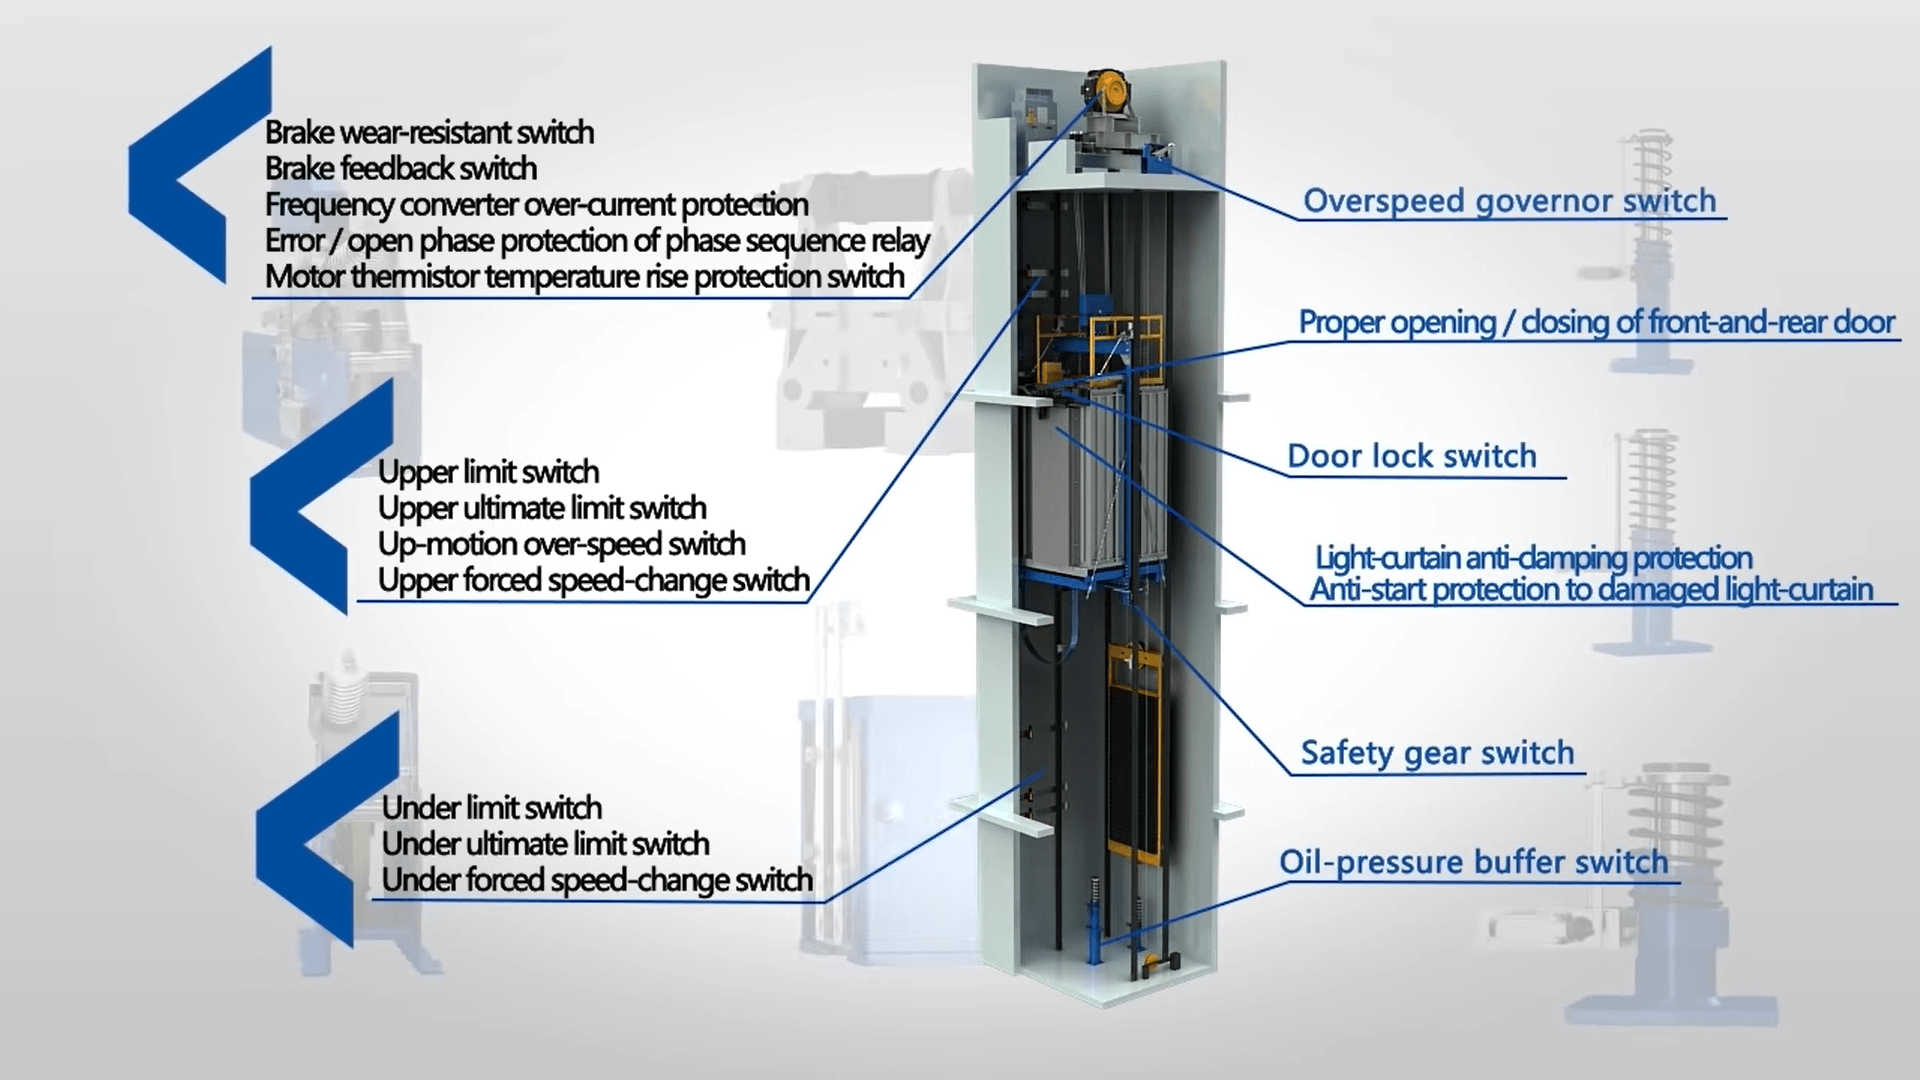
\includegraphics[width=1\linewidth]{img/safety_gaurantees}
		\caption{Modern elevators safety gears}
		\label{fig:safetygaurantees}
	\end{figure}
 
 	\begin{wrapfigure}{L}{0.4\textwidth}
 		\begin{center}    		
 			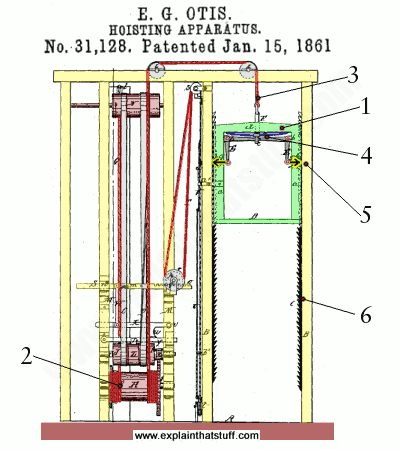
\includegraphics[scale=1.8]{img/Otis_elevator_principle}
 		\end{center}
 		\caption*{Otis's safety hoist}
 	\end{wrapfigure}
 	The graph in the left illustrate the principle that Otis's safety hoist 
 	applied. The main idea is that when the rope breaks, the arms marked by 4 
 	in the graph will be ejected (Newton's 2nd law of motion), thus preventing 
 	it from directly plummeting to bottom.
 	
 	Yeah, this is the prototype of early elevators, ugly though, the Woolworth 
 	Building\footnote{The Woolworth Building is an early American 
 	skyscraper designed by architect Cass Gilbert and located at 233 Broadway 
 	in Manhattan, New York City. It was the tallest building in the world from 
 	1913 to 1930, with a height of 792 feet (241 m). More than a century after 
 	its construction, it remains one of the 100 tallest buildings in the 
 	United States.} adopted this elevator system and made itself the tallest 
 	building in the world from 1913 to 1930. 
	
	Of course, modern elevators (see
	 \hyperref[fig:safetygaurantees]{figure 1}) 
	are much more advanced than it. They possess 
	\emph{multiple safety guarantees}. As we shall 
	see, a modern elevator generally has a 
	\emph{counterweight} on the other end of 
	the rope to offset the weight of car so that
	the motor has an easier job moving the elevator
	load. It usually about half the weight 
	of a fully loaded passenger elevator. So, 
	on an average ride, the two are 
	perfectly balanced. All the motor needs 
	to do to move the car is provide a 
	nudge to tip the balance one way or 
	the other. This system saves energy as 
	well as wear and tear on moving parts.
	Once the car is moving, the motor's 
	only job is to control
	one of the two falling objects.
	Both the car and counterweight are
	attached to guide rails inside the shaft,
	they keep everything from swaying back
	and forth and also give a backup set of
	brakes something to grab onto. If
	anything goes wrong with the motor,
	Hydraulic fluid is cut off and that
	automatically releases this brake that
	seizes the ropes for a quick stop.
	Technically one of these steel ropes is
	enough to hold up both the car and the
	counterweight, the rest are there for
	backup in case one snaps. Even if the
	whole set is cut, don't worry, it still
	won't plummet since this machine has a
	built-in fail-safe. There's a 
			\hyperref[governor]{governor\footnote{
			The governor, which is located in the machine room or 
			overhead depending on the elevator design, is a speed monitoring 
			device on traction elevators that triggers the safety mounted on 
			the car frame when the elevator over-speeds in either direction.}} 
	located beside the motor with its own
	pulley and separate cable attached to
	the car. There are two spring-loaded
	metal hooks (see \hyperref[governor]{
	figure 2 subfigure (a)}) called
	fly weights inside the governor. If a
	car-free falls and the governor spins
	too fast, centrifugal force pushes the
	hooks out. They cease ratchets on the
	fixed inner rim and stop the pulley. the
	governor's rope jerks on an arm on top
	of the car and this locks the brakes.
	
	The idea of the rope elevator is simple
	enough - one side goes up the other goes
	down. It just took a couple of thousand
	years to figure out how to stop it.
	It's easy enough to drive but without
	breaks we'd rather walk. (View YouTube
	video \textit{How Elevator Works}
	\href{https://markjohntaylor.com/blog/wordpress/index.php/2020/06/15/the-elevator#principle}
	{here}
	, and view YouTube video \textit{Elevator Brake Systems} 
	\href{https://markjohntaylor.com/blog/wordpress/index.php/2020/06/15/the-elevator#brake}{here})
	
	\begin{figure}
		\makebox[\textwidth][c]{			
			\subfloat[{governor unlocked}
			]{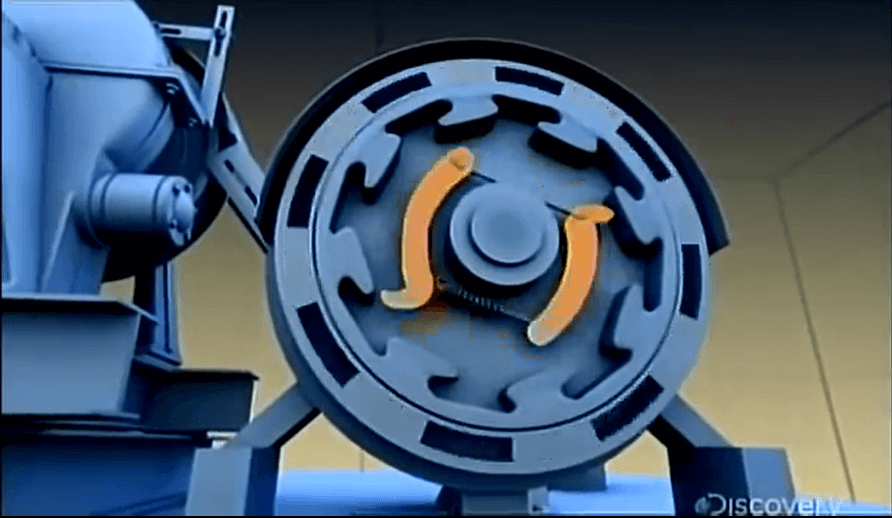
\includegraphics[width=0.5\textwidth]{img/governor_unlocked_1}}
			\subfloat[{governor locked}
			]{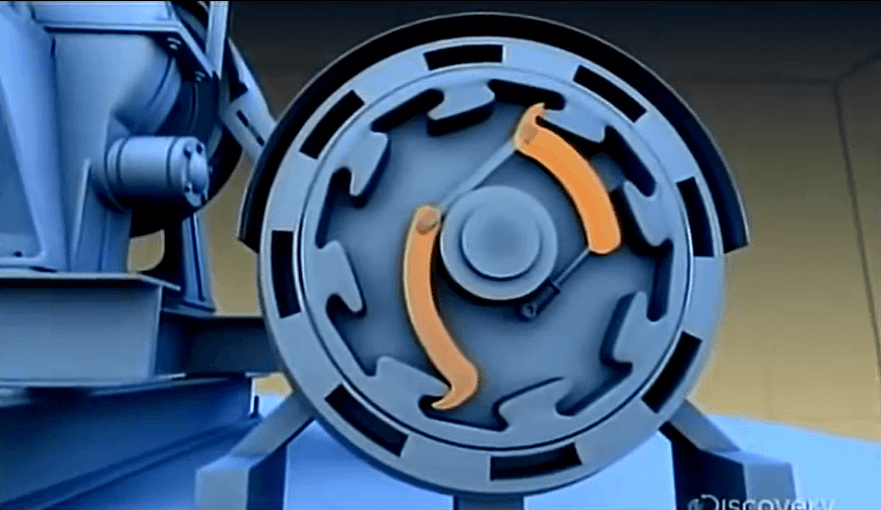
\includegraphics[width=0.5\textwidth]{img/governor_locked_1}
		}}\\
		\makebox[\textwidth][c]{			
			\subfloat[{another version: governor unlocked}
			]{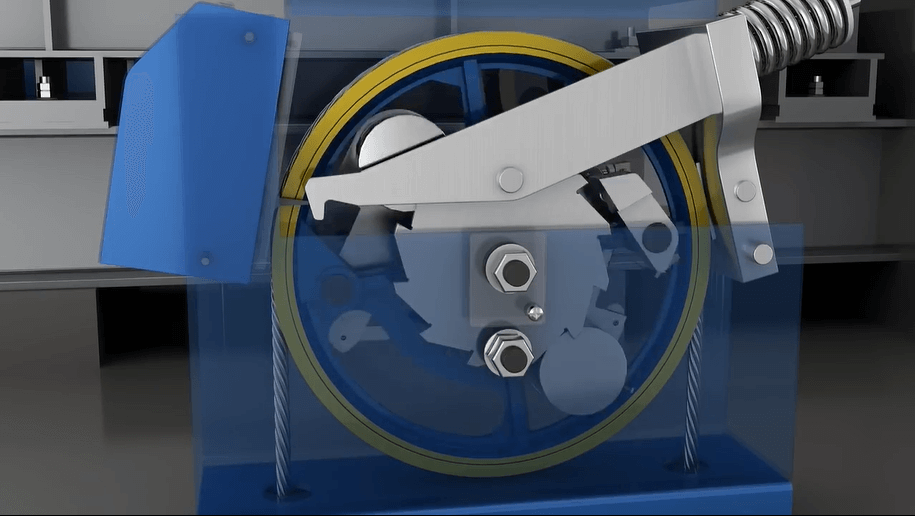
\includegraphics[width=0.5\textwidth]{img/governor_unlocked_2}}
			\subfloat[{another version: governor locked}
			]{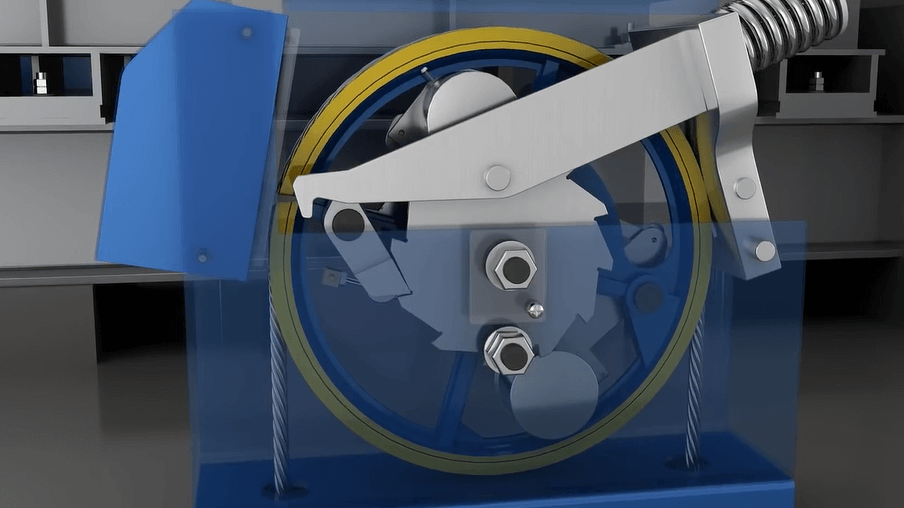
\includegraphics[width=0.5\textwidth]{img/governor_locked_2}
		}}		
		\caption{Governor locks when overspeed is detected}
		\label{governor}
	\end{figure}
	
	\clearpage
	